\documentclass[tikz,border=1pt]{standalone}

\usepackage{amsmath}

\begin{document}
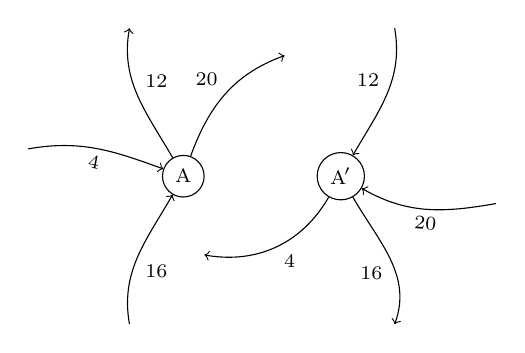
\begin{tikzpicture}[auto,scale=2]\scriptsize
	\node[circle,draw] (N1) {A};
	\node[circle,draw] at (1,0) (N2) {$\text{A}\mkern-2mu'$};

	\draw[->] (N1) to[out=120,in=-100]	node[swap]		{12}  +(110:1);
	\draw[<-] (N2) to[out=60,in=-80]	node[]			{12} +( 70:1);
	\draw[<-] (N1) to[out=160,in=10]	node[swap,sloped]	{4}  +(170:1);
	\draw[->] (N2) to[out=240,in=-10]	node[]			{4}  +(210:1);
	\draw[<-] (N1) to[out=-120,in=100]	node[]			{16}  +(250:1);
	\draw[->] (N2) to[out=-60,in=70]	node[swap]		{16} +(-70:1);
	\draw[->] (N1) to[out=70,in=200]	node[]			{20} +( 50:1);
	\draw[<-] (N2) to[out=-30,in=190]	node[sloped,swap]	{20} +(-10:1);
\end{tikzpicture}
\end{document}
